\chapter{Descrizione software}
\label{ch:interface}


Il software è diviso in tre componenti principali:
\begin{enumerate} [nolistsep]
    \item un ambiente grafico per la gestione dei parametri iniziali,
    \item l'algorirmo di simulazione,
    \item alcuni strumenti grafici per la visualizzazione dei risultati.
\end{enumerate}
Ognuna di queste componenti è indipendente dalle altre, poiché le informazioni sono passate attraverso file che vengono ogni volta aggiornati, in questo modo è sempre possibile risalire ai parametri utilizzati, modificarli senza usare l'ambiente grafico e gestire tutto da riga di comando.
In figura (\ref{fig:schema}) è riassunto lo schema di funzionamento. Si crea tramite l'interfaccia un file \textsl{Par.py} che riassume tutti i parametri iniziali, si lancia la simulazione dall'interfaccia, l'algoritmo simulativo salva i risultati in una cartella precedentemente selezionata. I risultati sono poi animati tramite un altro strumento grafico. Si noti che da riga di comando è possibile lanciare in maniera indipendente sia l'algoritmo simulativo sia gli strumenti di animazione, basta che siano presenti i file intermedi necessari.

Il codice è stato scritto utilizzando il linguaggio Python appoggiandosi alle librerie esterne:
\begin{itemize}[nolistsep]
    \item Numpy, per le funzioni matematiche e la gestione dei vettori,
    \item Matplotlib, per generare i grafici e le animazioni,
    \item Tkinter, per la costruzione dell'interfaccia grafica,
    \item Numba, per compilare le funzioni di evoluzione temporale.
\end{itemize}

\textcolor{red}{
Per visualizzare i risultati, oltre che al semplice strumento di animazione, sono stati implementati:
\begin{itemize}[nolistsep]
	\item uno strumento per confrontare le soluzioni numeriche con le soluzioni analitiche, 
	\item uno strumento per visualizzare l'evoluzione in contemporanea nello spazio diretto e nello spazio dei momenti,
	\item uno strumento per il calcolo dei coefficienti di riflessione e di trasmissione.
	\item uno strumento per il calcolo dei valori medi
	\item uno struemento per la valutazione dell'errore rispetto alla funzione analitica 
\end{itemize}
}

\begin{figure}
    \centering
    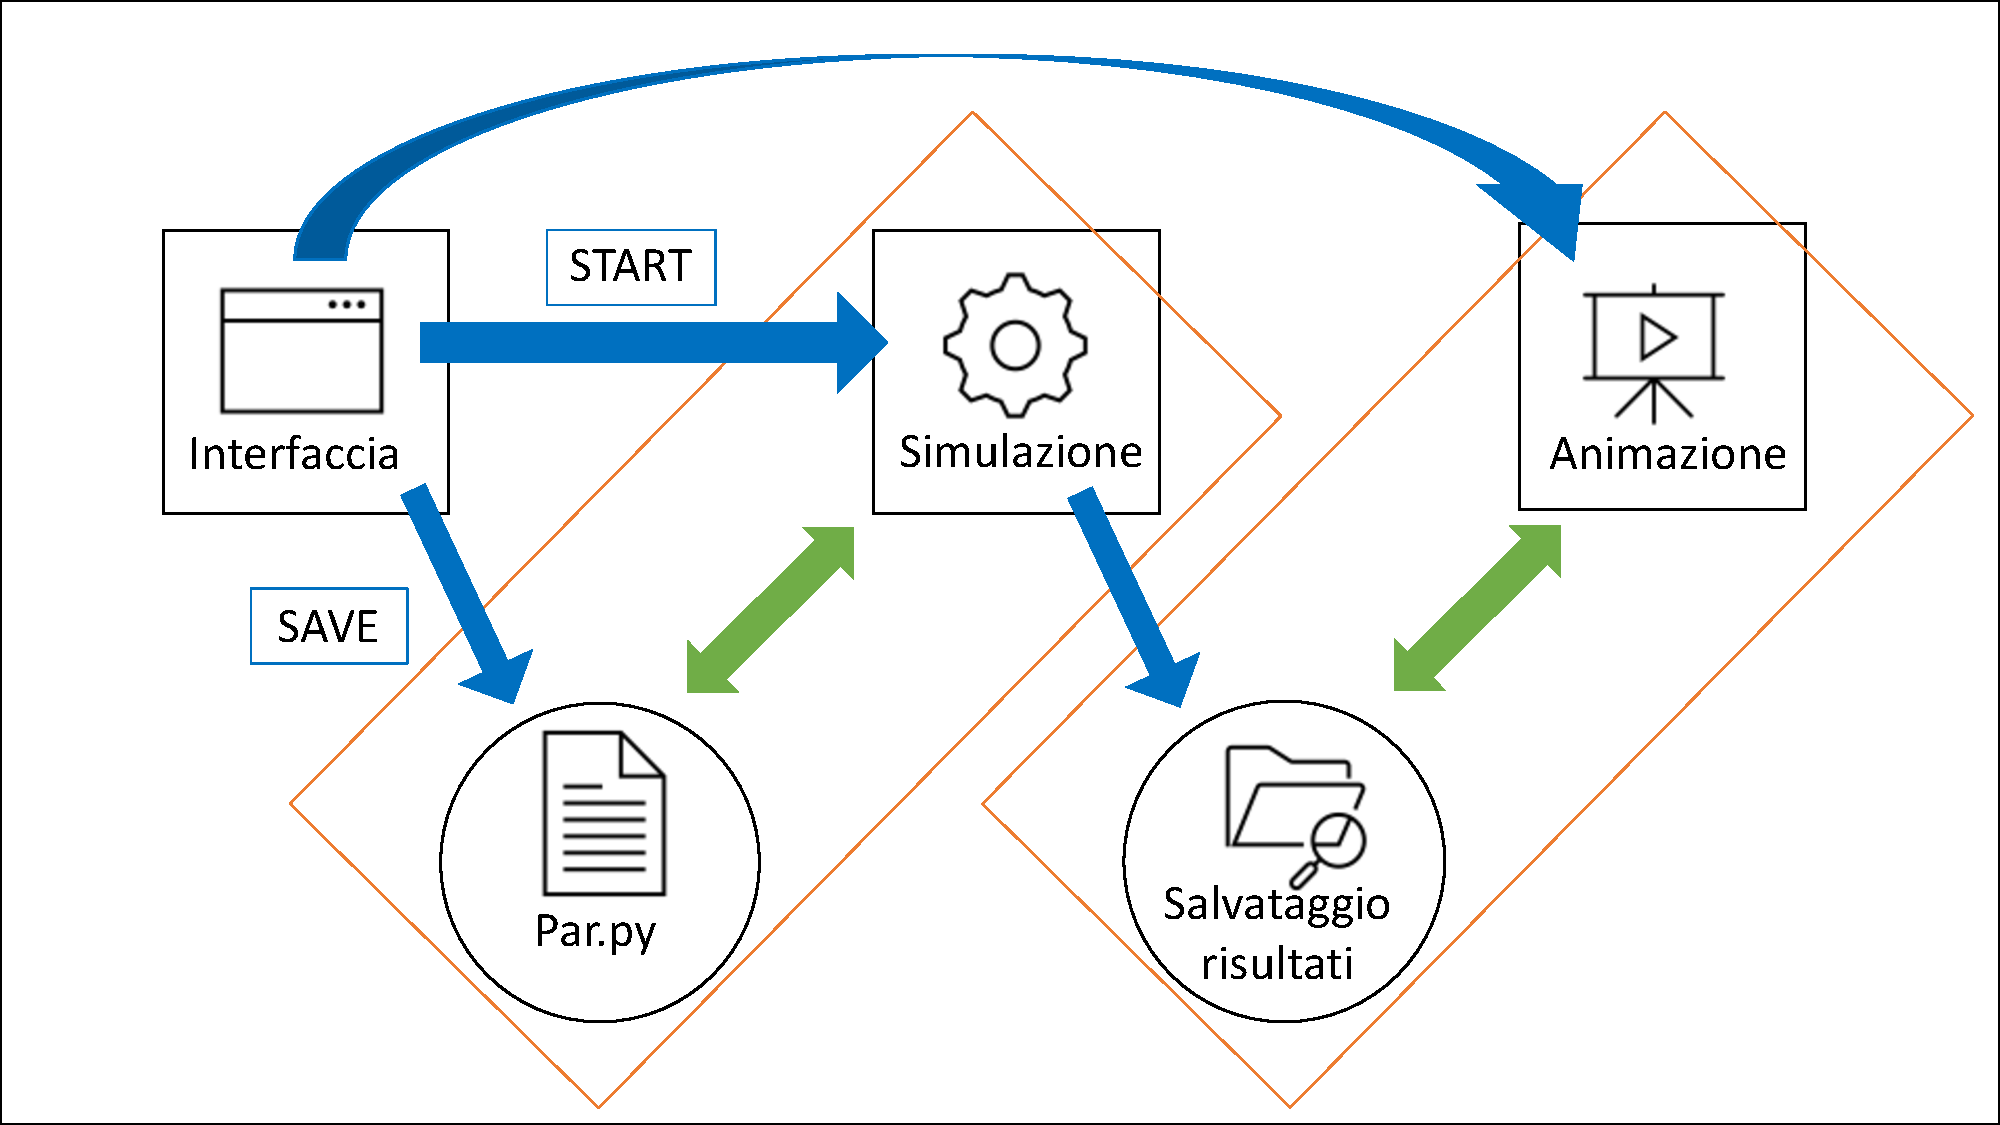
\includegraphics[width = 0.6\textwidth]{immagini/schema.pdf}
    \caption{Schema di funzionamento del software. \textcolor{red}{È una bozza se mi conferma che può andare bene la perfeziono}}
    \label{fig:schema}
\end{figure}

\begin{figure}
    \centering
    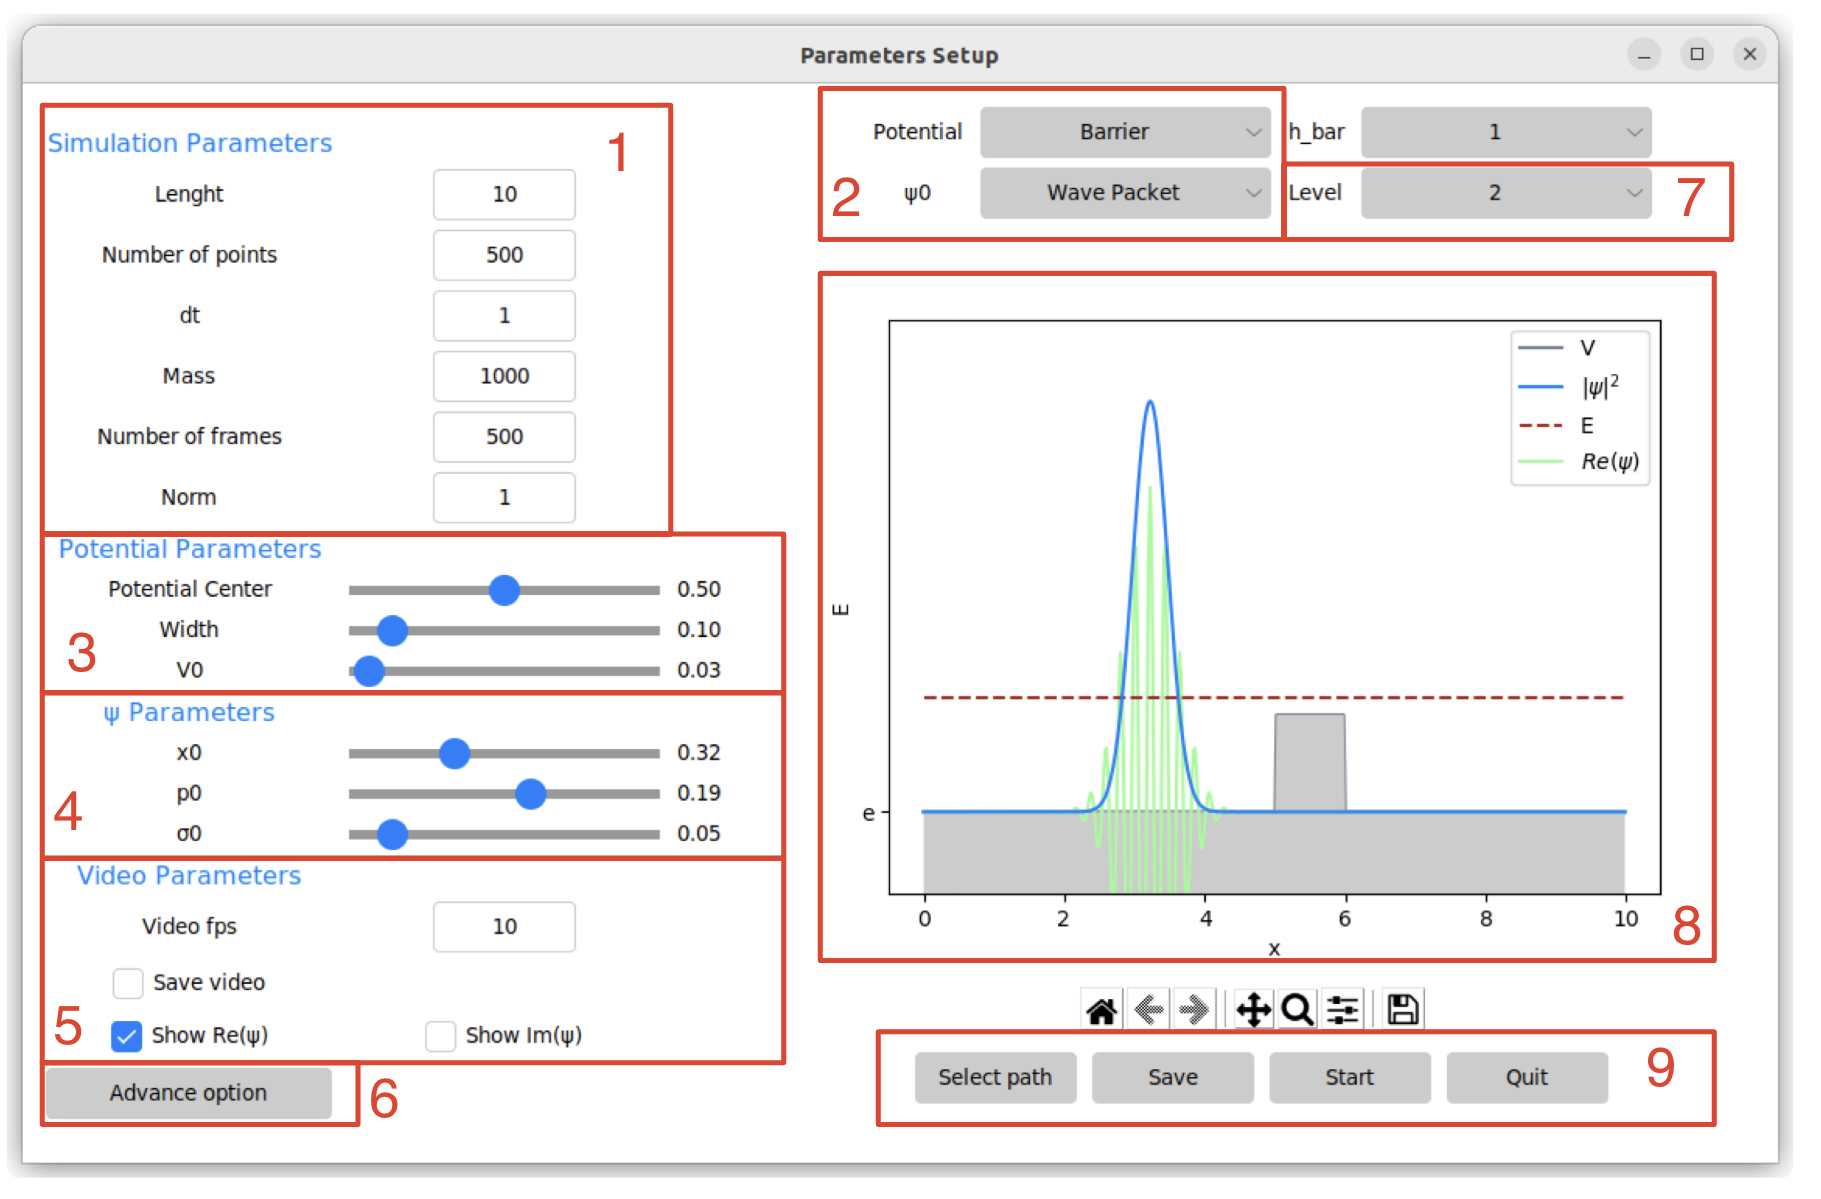
\includegraphics[width = 0.7\textwidth]{immagini/inter_num.jpg}
    \captionsetup{singlelinecheck=off}
    \caption[foo bar]{Illsustrazione dell'interfaccia.
    \small{
    \begin{enumerate}[nolistsep]
        \item Si possono modificare i parametri caratteristici dello spazio e della particella, nonché impostare il numero e la grandezza dei passi temporali da eseguire.
        \item Permette di scegliere tra gli stati e i potenziali citati al capitolo (\ref{ch:applicazioni}).
        \item È possibile modificare i parametri caratteristici del potenziale selezionato.
        \item È possibile modificare i parametri caratteristici dello stato iniziale selezionato. Quando si modificano parametri che influenzano la funzione d'onda nello spazio dei momenti viene messa in mostra un'anteprima dello stato iniziale nello spazio dei momenti. 
        \item  Si possono modificare alcuni parametri per la creazione dell'animazione finale. Tra questi è possibile mostrare la parte reale e immaginaria della soluzione.
        \item Tra le opzioni avanzate si può selezionare l'algoritmo di simulazione, vedi sezione (\ref{sec:ev_code}), e inserire dei controlli per la conservazione della norma e dell'energia.
        \item Il parametro  \textsl{Level} indica l'ordine a cui viene troncata l'espansione in eq. (\ref{eq:LT_expantion}).
        \item Viene visualizzata in diretta un'anteprima dello stato iniziale.
        \item Cliccando sui seguenti tasti si controllano le funzioni dell'interfaccia. Per eseguire in maniera corretta la simulazione la procedura prevista è: selezionare il percorso di salvataggio, salvare i risultati, far partire la simulazione e attendere l'animazione, uscire.    
    \end{enumerate}
    } }
    \label{fig:interface}
\end{figure}

\section{Algoritmo di simulazione}
\label{sec:ev_code}

Il cuore dell'algoritmo di simulazione è un ciclo che richiama ad ogni iterazione una funzione di evoluzione e salva i risultati nella cartella indicata dall'utente.
Sono state implementate tre diverse funzioni di evoluzione che differiscono per generalità e prestazioni. Inoltre l'utente può scegliere tra due tipologie di algoritmi di simulazione: con o senza anteprima, dove con anteprima si intende una visualizzazioni in diretta dei risultati della simulazione. Questa scelta è dovuta alla perdita di velocità causata dalla creazione immediata dei grafici.
Di seguito si riporta il codice utilizzato per la più generica funzione di evoluzione, con la quale è possibile simulare un potenziale dipendente dal tempo e selezionare l'ordine a cui viene troncata l'espansione.
\begin{lstlisting}[language = Python]
@jit
def evolution_t_dependent(y, q, k, dt, V, m, mat_f, mat_i, 
            N, L, h, P_MAX, f_zero, coefficients, Level):
    for i in range(Level):
        if coefficients[i][0] != 0:
            # V terms application
            y = exp_V(y, V, dt, h, coefficients[i][0])
        if coefficients[i][1] != 0:
            # Fourier transform 
            f_y = DFT.Dft(y ,q, k, mat_f, N, L, h, f_zero)   

            f_y = DFT.shift(f_y, k, P_MAX)
            k = DFT.shift_p(k, P_MAX)

            # T terms application
            f_y = exp_T(f_y, k, m, dt, h, coefficients[i][1])      

            f_y = DFT.back_shift(f_y, k)
            k = DFT.back_shift_p(k, P_MAX)

            # Anti-Fourier transform
            y= DFT.iDft(f_y, q, k, mat_i, L, h, f_zero)   
    return y
\end{lstlisting}
Il simbolo \textsl{@jit} è detto \textsl{decorator} e serve per compilare la funzione attraverso Numba. Tale processo rende il calcolo molto più rapido, ma per poter sfruttare al meglio le potenzialità di questo compilatore bisogna rinunciare ad alcune comodità tipiche dei linguaggi interpretati come Python. Numba richiede, infatti, che tutte le variabili utilizzate nella funzione siano passate come parametri e che le variabili siano di tipo statico. Per questo vengono inseriti tra i parametri alcuni termini che non hanno a che fare con l'evoluzione del sistema, ma che sono utilizzati come variabili di appoggio, come ad esempio \textsl{f\_zero}.
DFT è la libreria personale utilizzata per raggruppare i metodi che computano la trasformata di Fourier. Si ricorda che per poter applicare i termini a cui esponente compare $\hat{T}$ oltre che applicare la trasformata di Fourier è anche necessario traslare la soluzione, questo viene fatto tramite i metodi \textsl{shift}, vedi sezione (\ref{sec:DFT}). Per rendere il codice più efficiente, le matrici, \textsl{mat\_f} e \textsl{mat\_i}, utilizzate per calcolare le trasformate sono precalcolate e vengono passate alle funzioni come parametri.
Il parametro \textsl{coefficients} rappresenta un vettore di dimensioni $Level \times 2$ che raggruppa i coefficienti $c_j$ e $d_j$ dell'espansione. 
Le funzioni \textsl{exp\_V} e \textsl{exp\_T} restituiscono semplicemente i termini esponenziali che compaiono nell'espansione. La funzione può essere resa più efficiente in quei casi in cui è possibile precalcolare alcuni termini. Per i potenziali non dipendenti dal tempo, infatti, i risultati resistituiti dalle funzioni \textsl{exp\_V} e \textsl{exp\_T} sono sempre gli stessi. Quindi risulta più efficiente precalcolari e passarli come parametri, in modo da dover eseguire solo una moltiplicazione. Con questa modifica si ottiene la seconda versione della funzione di evoluzione.
Rinunciando ad un ulteriore grado di libertà si può rendere la funzione ancora più efficiente. Infatti e prestazioni del compilatore Numba sono infatti piuttosto sensibili alla presenza di condizioni \textsl{if} e di condizioni sui cicli. Se si elimina il ciclo \textsl{for} per sostituirlo con una serie operazioni da eseguire tutte in fila e si eliminano manualmente i termini nulli si ottiene un considerevole aumento nelle prestazioni. Per poter implemenatare una tale funzione è quindi necessario conoscere in precedenza sia il livello sia i coefficienti associati a tale livello. Nel codice è stato implementata una funzione di quest'ultimo tipo per il livello che corrisponde a troncare l'espansione a $O(\delta t^{\, 3})$.




